\documentclass{report}
\usepackage{graphicx}
\usepackage[table]{xcolor}
\begin{document}

\title{Tugas Mata Kuliah Kecerdasan Buatan Chapter 2}
\maketitle

{\bf Muhammad Nazhim Maulana (1194025)}
\vspace{0.4cm}

{\bf \emph{Binary Classification}}
\vspace{0.1cm}
\\\hangindent=0.5cm \emph{Binary Classification} merupakan salah satu bentuk klasifikasi yang dimana data-data yang diklasifikasikan itu hanya dibagi menjadi dua buah kelas saja. Jadi klasifikasi ini sama halnya dengan memprediksi dikelompok manakah satu benda itu berada. Klasifikasi ini hanya membagi data menjadi dua kelompok saja dan tidak lebih.

\vspace{0.4cm}
\begin{center}
Tabel Ilustrasi \emph{Binary Classification} 
\begin{table}[h!]
\centering
\begin{tabular}{|c|l|l|l|l|} % Membuat garis vertikal
\hline % Membuat garis horizontal pertama
No. & Aplikasi &  Label A& Label B \\
\hline % Membuat garis horizontal kedua
1   & Diagnosa Kesehatan & Sehat & Sakit\\
2   & Analisa Email & Tidak Spam & Spam\\
3   & Analisa Keuangan & Tidak Curang & Curang\\
4   & Pemasaran&	Tidak Beli& Beli\\
\hline % Membuat garis horizontal ketiga
\end{tabular}
\end{table}
\end{center}

\begin{figure}[hbtp]
\caption{Gambar Ilustrasi}
\centering
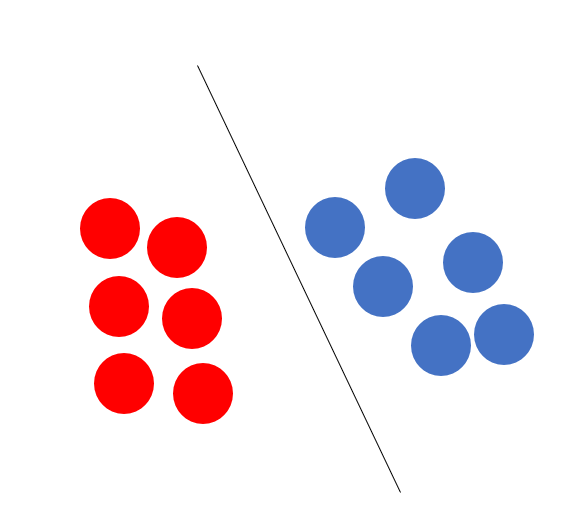
\includegraphics[scale=0.6]{../figures/Ilustrasi.png}
\end{figure}

\vspace{0.1cm}
\hangindent=0.5cm Pada tabel dan juga gambar diatas dapat dilihat  dengan jelas bagaimana \emph{Binary Classification} itu. Dapat dilihat bahwa pembagian kelompok setiap benda pasti hanya akan menjadi dua saja apakah A atau B dan tidak ada satu kelas tambahan yang lainnya.

\vspace{0.5cm}

{\bf \emph{Supervised}, \emph{Unsupervised Learning}, dan \emph{Clustering}}
\vspace{0.1cm}
\\\hangindent=0.5cm \emph{Supervised Learning} adalah salah satu jenis dari algoritma yang digunakan untuk mengajar sebuah \emph{Machine Learning}, untuk pembelajarannya ini akan diawasi langsung oleh seorang \emph{Supervisor} atau pengawas. Algoritma ini akan memerlukan sebuah data berlabel untuk membangun model yang memiliki tingkat akurasi yang terus menerus dapat ditingkatkan.

\vspace{0.4cm}
\hangindent=0.5cm Seperti yang telah dijelaskan pada chapter satu sebelumnya, \emph{Unsupervised Learning} merupakan kebalikan dari  \emph{Supervised Learning}. Jikalau \emph{Supervised Learning} itu memiliki pengawas, maka \emph{Unsupervised Learning} sendiri tidak diawasi. Dengan begitu algoritma ini cenderung lebih bebas dalam proses eksplorasi data karena tiap data yang ada tidak memiliki label sehingga lebih mudah dalam melakukan eksplorasi dan menemukan data yang tersembunyi.

 \begin{figure}[hbtp]
 \caption{Analogi Supervised Learning}
 \centering
 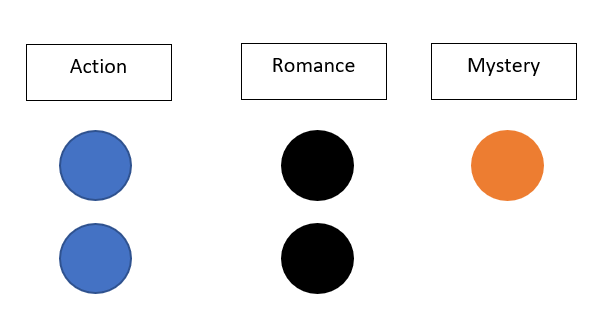
\includegraphics[scale=0.4]{../figures/supervised learning.png}
 \end{figure}
 
 \begin{figure}[hbtp]
 \caption{Analogi Unsupervised Learning}
 \centering
 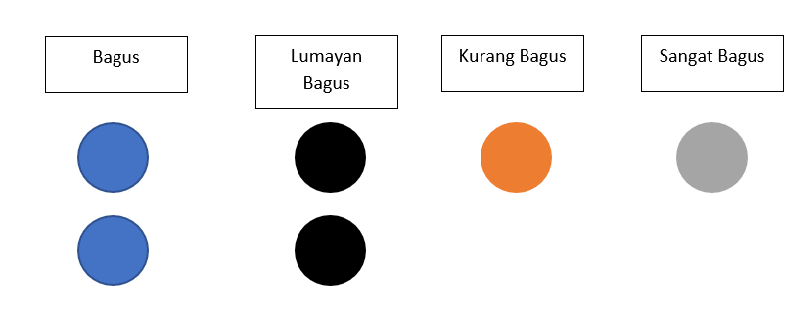
\includegraphics[scale=0.4]{../figures/unsupervised learning.png}
 \end{figure}
 
 \hangindent=0.5cm Perhatikan dua buah gambar diatas. keduanya merupakan analogi dari \emph{Supervised Learning} dan \emph{Unsupervised Learning}. Ketika mendownload beberapa film kemudian menyimpannya ke dalam folder berdasarkan genre, dengan begitu kita bisa langsung dengan mudah menyimpan film baru ke dalam folder yang di awal tadi telah dibuat karena genre dari filmnya juga diketahui. 
 
 \vspace{0.3cm}
 
\hangindent=0.5cm Itu untuk \emph{Supervised Learning}, sedangkan untuk \emph{Unsupervised Learning}, genre tadi tidak ada maka film-film akan dikelompokkan secara acak karena tidak ada label yang disediakan untuk membedakan film-film itu maka dibuatlah label-label baru seperti Bagus, kurang bagus dan sebagainya. Dari penjelasan tadi maka dapat dilihat dengan cukup jelas mengenai perbedaan antara \emph{Supervised} dan \emph{Unsupervised Learning}

\vspace{0.4cm}
\pagebreak{}
\begin{figure}[t!]
\centering
\caption{Ilustrasi clustering}
\centering
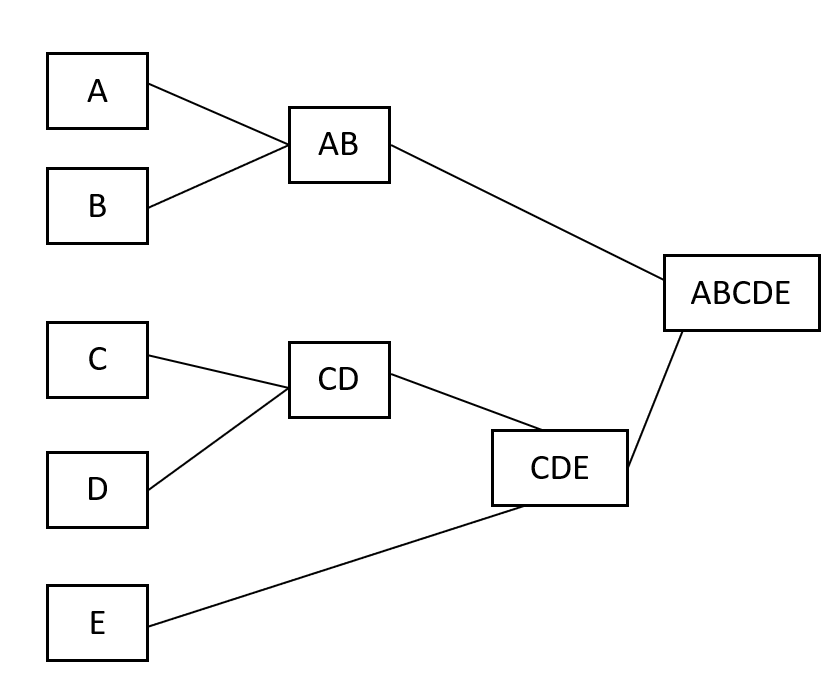
\includegraphics[scale=0.3]{../figures/Clustering.png}
\end{figure}


\hangindent=0.5cm \emph{Clustering} adalah proses pengelompokkan data ke dalam beberapa \emph{cluster} atau kelompok, dengan begitu dalam satu \emph{cluster} memiliki tingkat kemiripan yang maksimum dan data antar \emph{cluster} yang berbeda memilipi kemiripan minimum. Seperti pada gambar diatas yang merupakan salah satu contoh clustering dari beberapa huruf. Pertama semua huruf berada pada kelompok yang berbeda-beda kemudian di kelompokkan lagi hingga ada kelompok dimana semua huruf ada.

\vspace{0.5cm}

{\bf Evaluasi dan Akurasi}
\vspace{0.1cm}

\begin{figure}[hbtp]
\centering
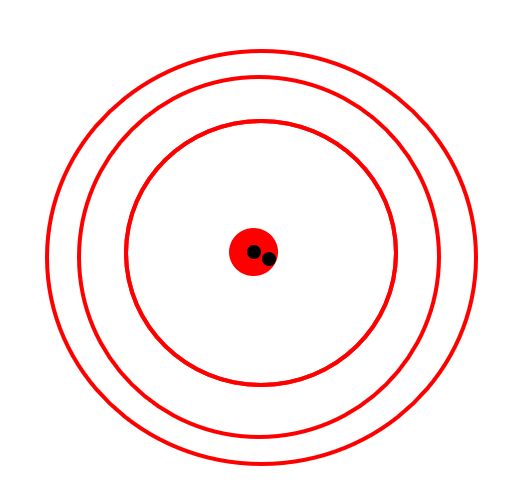
\includegraphics[scale=0.3]{../figures/Accuracy and Evaluation.png}
\caption{Accuracy}
\end{figure}

\vspace{0.1cm}

\hangindent=0.5cm Berdasarkan buku, evaluasi adalah penilaian yang dilakukan untuk mengukur seberapa baik keakuratan dari sebuah model. Dengan adanya evaluasi maka kesalahan-kesalahan yang dibuat oleh model bisa dilihat dan juga di analisis. Untuk Akurasi sendiri, merupakan sebuah pengukuran yang penting untuk dilakukan selama melatih sebuah model atau mesin dan juga untuk melihat seberapa baik hasil akhir yang diperoleh dari sebuah mesin.

\vspace{0.5cm}

{\bf Membuat dan Membaca \emph{Confusion Matrix}}
\vspace{0.1cm}
\\\hangindent=0.5cm \emph{Confusion Matrix} adalah pengukuran performa klasifikasi \emph{machine learning} dengan keluaran berupa dua kelas atau lebih. \emph{Confusion Matrix} berisi tabel dengan empat kombinasi berbeda dari nilai prediksi dan nilai aktual. Ada empat istilah dalam \emph{Confusion Matrix} yaitu:

\begin{enumerate}
  \item \emph{True Positive} (TP)
   \\\hangindent=0.5cm Artinya prediksi yang dibuat itu positif dan memang benar
  
  \item \emph{True Negative} (TN)
   \\\hangindent=0.5cm Artinya prediksi yang dibuat itu negatif dan memang benar
   
  \item \emph{False Positive} (FP)
   \\\hangindent=0.5cm Artinya prediksi yang dibuat itu positif dan salah
   
  \item \emph{False Negative} (FN)
   \\\hangindent=0.5cm Artinya prediksi yang dibuat itu negatif dan memang salah
   
\end{enumerate}

\vspace{0.4cm}
\begin{center}
Tabel Ilustrasi \emph{Confusion Matrix} 
\begin{table}[h!]
\centering
\begin{tabular}{|c|l|l|l|l|} % Membuat garis vertikal
\hline % Membuat garis horizontal pertama
n = 175 & Aktual: Positif (1) &  Negatif (0) \\
\hline % Membuat garis horizontal kedua
Prediksi: Positif (1)   & TP: 125 & FP: 20\\
\hline 
Prediksi: Negatif (0)   & FN: 25 & TN: 5\\
\hline 
   & 150 & 25\\
\hline % Membuat garis horizontal ketiga
\end{tabular}
\end{table}
\end{center}

\hangindent=0.5cm Sebagai sebuah disini ada sebuah perusahaan yang membuat model untuk membuat prediksi apakah karyawan di perusahaan tersebut terjangkit covid-19 atau tidak. Diasumsikan bahwa terdapat 175 karyawan dengan prediksi 145 karyawan dan yang negatif sebanyak 30 namun pada kenyataannya yang positif ada 150 dan yang negatif ada 25 orang.

\vspace{0.5cm}

{\bf K-fold \emph{Cross Validation}}
\vspace{0.1cm}

\hangindent=0.5cm \emph{Cross Validation} Merupakan sebuah teknik validasi dari pengambilan model \emph{Split Validation} dimana validasinya mengukur \emph{training error} dengan menguji data uji. Untuk contoh dari \emph{Cross Validation} dapat dilihat seperti pada gambar tabel yang ada di bawah ini.

\vspace{0.4cm}
\begin{center}
Tabel Ilustrasi \emph{Cross Validation}
\begin{table}[h!]
\centering
\begin{tabular}{|c|l|l|l|l|} % Membuat garis vertikal
\hline % Membuat garis horizontal pertama
Percobaan 1&\cellcolor{orange!50} Test  &  Test & Test & Test \\
\hline % Membuat garis horizontal kedua
Percobaan 2& Test & \cellcolor{orange!50}Test & Test & Test\\
\hline 
Percobaan 3&Test & Test &\cellcolor{orange!50} Test & Test \\
\hline 
Percobaan 4&Test & Test & Test &\cellcolor{orange!50} Test \\
\hline % Membuat garis horizontal ketiga
\end{tabular}
\end{table}
\end{center}

\vspace{0.5cm}

{\bf \emph{Decision Tree}}
\vspace{0.1cm}

\hangindent=0.5cm \emph{Decision Tree} Merupakan sebuah alat yang menjadi pendukung dengan struktur yang mirip dengan pohon untuk memodelkan kemungkinan hasil dan juga hingga kemungkinan konsekuensi yang mungkin dapat terjadi ketika mengambil atau memilih salah satu hal yang bisa saja berpengaruh dengan keadaan kita kedepannya. Untuk salah satu ilustrasinya dapat dilihat pada gambar berikut ini:

\begin{figure}[hbtp]
\caption{Contoh Decision Tree}
\centering
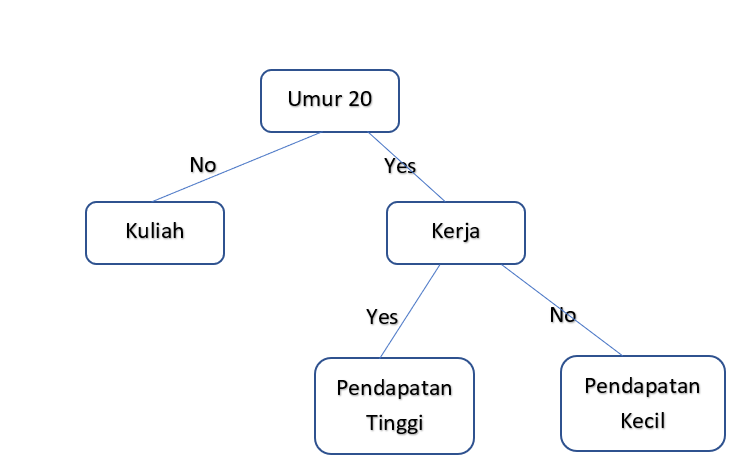
\includegraphics[scale=0.6]{../figures/Decision Tree.png}
\end{figure}

\vspace{0.5cm}

{\bf \emph{Information Gain} dan Entropi}
\vspace{0.1cm}

\hangindent=0.5cm \emph{Information Gain} adalah ukuran efektivitas satu atribut dalam mengklasifikasikan data dan biasanya digunakan untuk menentukan urutan atribut yang atributnya memiliki nilai informasi yang terbesar. Kemudian ada entropi yang merupakan informasi yang menyatakan ukuran ketidakpastian dari atribut dari satu kumpulan objek dalam satuan bit. Untuk setiap latihannya disini saya menggunakan variabel nama kota karena hasil mod dari NPM saya adalah 1 dan berikut adalah hasil-hasilnya:

\begin{enumerate}
  \item \emph{Load Dataset}
   \\\hangindent=0.5cm Berikut adalah hasil untuk load data setnya
   
   \begin{figure}[hbtp]
   \caption{Hasil Load Dataset}
   \centering
   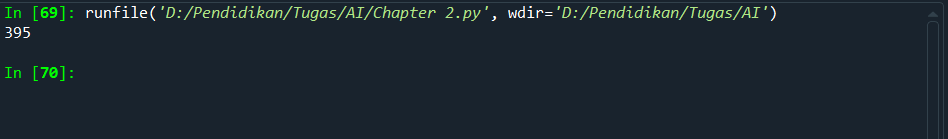
\includegraphics[scale=0.6]{../figures/Chapter 2 (1).PNG}
   \end{figure}
   
  
  \item \emph{Generate Binary Label}
   \\\hangindent=0.5cm Untuk praktikum yang kedua hasilnya adalah sebagai berikut:
   
   \begin{figure}[hbtp]
   \caption{Menabhakan Binary Label}
   \centering
   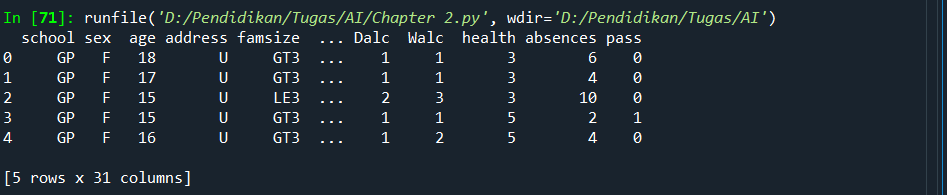
\includegraphics[scale=0.5]{../figures/Chapter 2 (2).PNG}
   \end{figure}
   
   
  \item \emph{Use encode on categorical column}
   \\\hangindent=0.5cm Selanjutnya melangkah ke praktikum yang ketiga dengan hasil seperti ini:
   
   \begin{figure}[hbtp]
   \caption{Hasil}
   \centering
   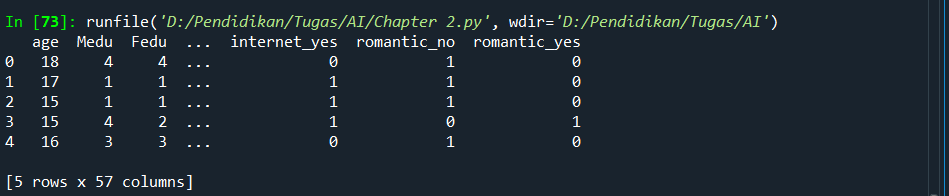
\includegraphics[scale=0.4]{../figures/Chapter 2 (3).PNG}
   \end{figure}
   
   
  \item \emph{Shuffle Rows}
   \\\hangindent=0.5cm Lanjut ke hasil praktikum yang selanjutnya yang hasilnya seperti pada gambar berikut ini:
   
   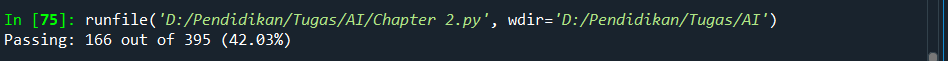
\includegraphics[scale=0.5]{../figures/Chapter 2 (4).PNG} 
   
  \item \emph{Visualize Tree}
   \\\hangindent=0.5cm Visulaize tree ini adalah memvisualisasikan decision tree yang sebelumnya itu telah dibuat

\vspace{0.5cm}

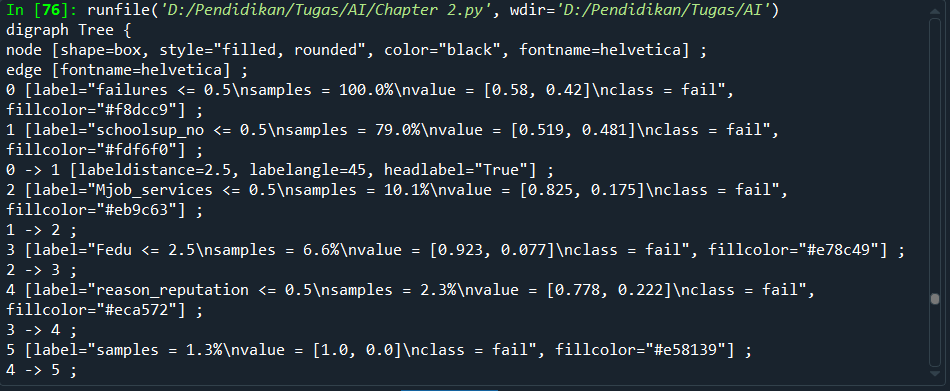
\includegraphics[scale=0.6]{../figures/Chapter 2 (5).PNG}    
   
     \item Praktikum 8
   \\\hangindent=0.5cm Untuk praktikum yang ketujuh hasilnya itu berupa dokumen saja yang isinya itu adalah hasil dari 
   
   
        \item \emph{Visualize Tree}
   \\\hangindent=0.5cm Visulaize tree ini adalah memvisualisasikan decision tree yang sebelumnya itu telah dibuat pada \emph{Visualize Tree} jadi langsung saja ke praktikum yang kedelapan yang hasilnya adalah seperti ini:
   
   \vspace{0.3cm}
   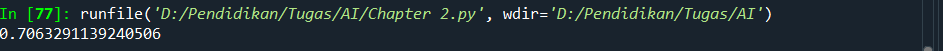
\includegraphics[scale=0.6]{../figures/Chapter 2 (6).PNG} 
   
        \item \emph{Accuracy}
   \\\hangindent=0.5cm Untuk praktikum mengenai Accuracy, hasilnya adalah seperti berikut ini:
   
   \vspace{0.5cm}
   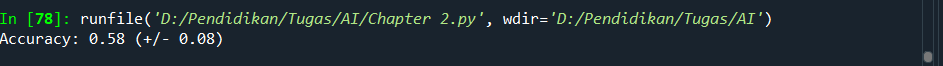
\includegraphics[scale=0.6]{../figures/Chapter 2 (7).PNG} 
   
        \item Praktikum 10
   \\\hangindent=0.5cm Untuk hasil dari praktikum 10 adalah sebagai berikut:

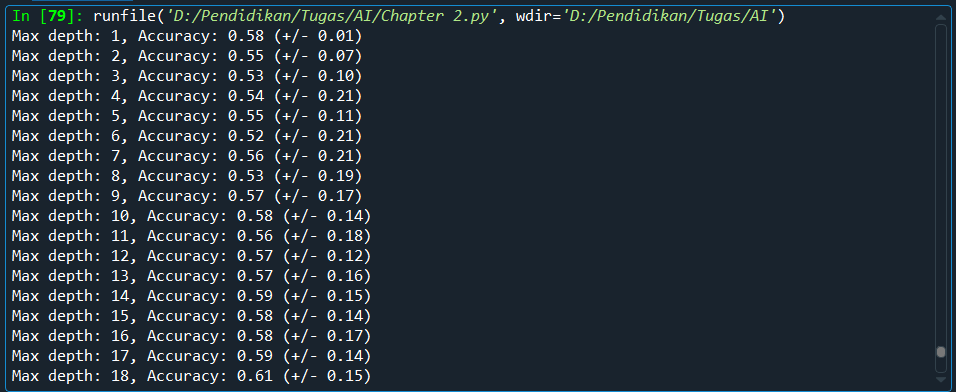
\includegraphics[scale=0.7]{../figures/Chapter 2 (8).PNG}    
   
        \item Praktikum 11
   \\\hangindent=0.5cm Praktikum 11 ini hasilnya adalah sebagai berikut:

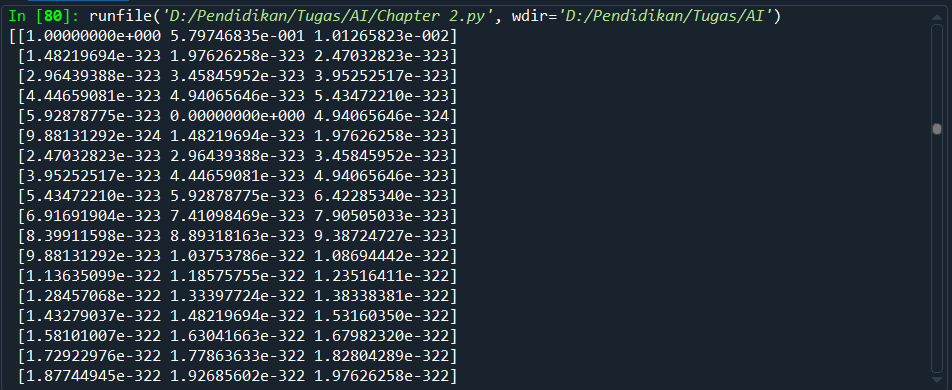
\includegraphics[scale=0.7]{../figures/Chapter 2 (9).PNG}    
   
        \item Praktikum 12
   \\\hangindent=0.5cm Praktikum 12 ini akan dibuat sebuah diagram dan hasilnya adalah sebagai berikut:

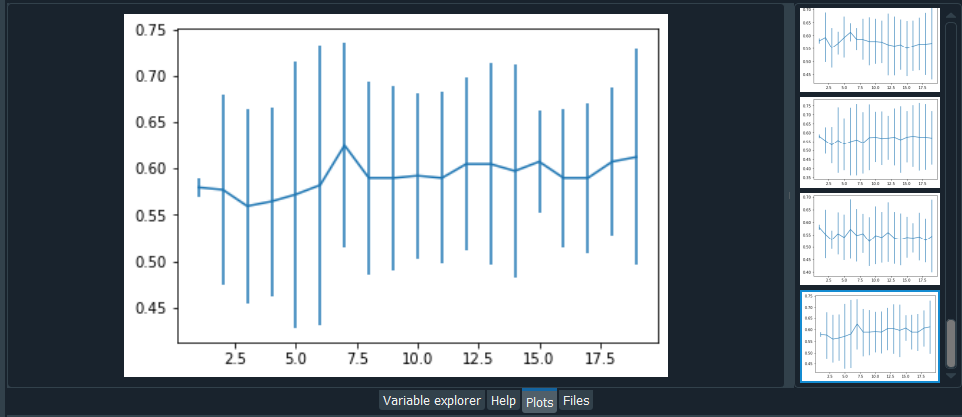
\includegraphics[scale=0.7]{../figures/Chapter 2 (10).PNG}       
      
\end{enumerate}

\vspace{0.5cm}

\hangindent=0.5cm Jadi untuk chapter 2 mulai dari teori hingga praktikum scikit-learnnya sudah selesai dikerjakan.

 \end{document}